% !TeX root = ../main.tex
% 原始章节：08-bus-and-soc.Rmd

\chapter{总线接口与SoC集成设计}\label{chap:08-bus-and-soc}

\section{计算机总线接口}\label{sec:08-bus-and-soc-001}

一个完整的计算机系统包含多个组成部件，这些部件通常由不同的设计人员或公司开发。为了使它们能够在一起协同工作，这些部件之间需要遵循一套共同的规则和规范，这种规范就是总线协议，总线协议是连接计算机系统中不同模块之间的桥梁。例如，计算机的主板可能由一家公司开发，而CPU由另一家公司设计。为了使这两个关键部件能够正常交互，它们之间就需要通过某种总线协议进行通信。总线协议规定了如何在连接线上传输数据，包括高电平、低电平分别代表什么含义，不同信号线之间的关系，数据传输的时序安排，以及如何进行数据校验和纠错。这些规定确保发送方能够将信息编码为适合传输的格式，通过总线传递，而接收方能够正确解读传输的信号。

总线的应用和标准化大幅简化了计算机系统的设计难度。通过引入统一的标准接口，制造商能够确保其设备可以与其他厂商的产品顺利协同工作，而无需为每个组件设计不同的连接方式。例如，某制造商生产的一块主板，只要符合相应的接口标准，就可以与任何支持该标准的CPU或其他硬件设备兼容。这种标准化不仅提升了各组件之间的兼容性，也大大优化了产品开发的流程。在工业领域，像PCI和USB这样的标准总线广泛用于各类计算机系统中。

从信号传输的方式来看，总线可分为并行总线和串行总线。并行总线通过多条传输线同时传输多个数据位，而串行总线则只通过一条传输线一次传输一位数据。并行总线的优势在于它能在相同频率下提供更大的数据传输带宽，因为多个比特能够并行传输。不过，并行传输要求所有数据位必须同步到达，这对总线的宽度、频率以及主板的设计提出了较高的要求。相比之下，串行总线采用单条传输线，每次传输一个比特，并通过编码技术将时钟信号嵌入数据中，使其能够以更高的频率进行数据传输。常见的并行总线包括类SRAM总线、AXI总线，而串行总线的代表则是USB、I2C等。

根据总线在计算机系统中的实际位置，可以将总线分为片上总线、内存总线、系统总线和设备总线。片上总线主要用于连接芯片内部的各个功能模块。在芯片设计过程中，通常会将其分为多个模块，这些模块间的数据交换依赖片上总线。例如，高性能的通用处理器可能包含多个处理器核、共享缓存和内存控制器，它们通过片上总线相互连接。而在片上系统（SoC）设计中，模块的数量和功能更为复杂，包括处理器核、内存控制器以及输入输出接口等，所有这些模块之间的通信都需要依赖标准的总线协议进行管理和协调。

本章将深入探讨类SRAM总线和AXI总线的设计原理以及它们在实际应用中的作用。

\section{类SRAM总线}\label{sec:08-bus-and-soc-002}

类SRAM总线是指一种类似于静态随机存取存储器（SRAM）接口的总线协议，适用于简单的存储访问场景。该节将详细介绍类SRAM总线协议的各个方面。

\subsection{主方和从方}\label{sec:08-bus-and-soc-003}

在类SRAM总线中，\textbf{主方（Master）}和\textbf{从方（Slave）}分别代表控制与被控制的设备：

\begin{itemize}
\tightlist
\item
  \textbf{主方（Master）：} 主方是发起操作的一方，它负责发起读或写请求，并与从方通信。
\item
  \textbf{从方（Slave）：} 从方被动接收来自主方的请求，并根据请求做出相应的操作，比如返回数据或接收数据。
\end{itemize}

为了方便理解，可以将从方理解为存储器，主方为希望对存储器进行操作的一方。

主从关系确保了通信的有序进行。主方控制通信过程的时序，而从方则根据主方的命令进行响应。在不同的应用场景下，可能会发生主从切换，即在某些情况下，原先的主方可能变为从方，反之亦然。

主方通过控制类SRAM总线的地址、数据和控制信号发起对从方的操作。通常，主方负责握手信号的发送，而从方则负责相应的反馈信号。当主从角色发生切换时，通常是为了平衡系统资源的使用或者在多主设备的系统中实现公平调度。

\subsection{接口信号}\label{sec:08-bus-and-soc-004}

类SRAM总线接口的信号设计是总线协议的重要部分，下表列举了类SRAM总线内的各个信号。
输出方向指的是由主方向从方传递的方向，输入方向指的是由从方向主方传递的方向。

\begin{longtable}[]{@{}llll@{}}
\toprule\noalign{}
信号 & 位宽 & 方向 & 功能 \\
\midrule\noalign{}
\endhead
\bottomrule\noalign{}
\endlastfoot
\texttt{clk} & 1 & - & 时钟 \\
\texttt{req} & 1 & 输出 & 请求信号,为1时有读写请求，为0时无读写请求 \\
\texttt{wr} & 1 & 输出 & 为1表示该次是写请求，为0表示该次是读请求 \\
\texttt{size} & 2 & 输出 & 该次请求传输的字节数 \\
\texttt{addr} & 32 & 输出 & 该次请求的地址 \\
\texttt{wstrb} & 4 & 输出 & 该次写请求的字节写使能 \\
\texttt{wdata} & 32 & 输出 & 该次写请求的写数据 \\
\texttt{addr\_ok} & 1 & 输入 & 该次请求的地址传输握手信号 \\
\texttt{data\_ok} & 1 & 输入 & 该次请求的数据传输握手信号 \\
\texttt{rdata} & 32 & 输入 & 该次请求返回的读数据 \\
\end{longtable}

相关重点信号的含义为：

\begin{itemize}
\item
  \textbf{\texttt{addr\_ok}}：由从方向主方发送该信号。在主方读时，该信号生效表示主方发送的地址\texttt{addr}已被从方接收；在主方写时，该信号生效表示主方发送的地址\texttt{addr}、数据\texttt{wdata}、字节写使能\texttt{wstrb}均被接收。
\item
  \textbf{\texttt{data\_ok}}：由从方向主方发送该信号。在主方读时，该信号生效表示从方返回的数据已通过\texttt{rdata}通道返回；在主方写时，该信号生效表示从方已经完成写入操作。
\item
  \textbf{\texttt{rdata}} 和 \textbf{\texttt{wdata}}：分别用于数据读取和写入，其中 \texttt{rdata} 是主方从从方接收到的读数据，而 \texttt{wdata} 是主方向从方传输的写数据。
\item
  \textbf{\texttt{size}}：表示一次数据传输的大小，通常为2位（如：00表示1字节，01表示2字节，10表示4字节，11表示8字节）。
\end{itemize}

\subsection{读写时序}\label{sec:08-bus-and-soc-005}

类SRAM总线的读写时序遵循一套标准的流程。以下将以一次读操作和一次写操作为例介绍。

\subsubsection{读操作}\label{sec:08-bus-and-soc-006}

在类SRAM总线上进行一次读事务时，主设备（Master）和从设备（Slave）之间的通信是通过一系列信号和时钟周期来完成的。图\ref{fig:sram-read}展示了一次类SRAM总线的读事务时序图，该图中展示的时序只是所有合法时序中的一种。

\begin{figure}[htbp]
  \centering
  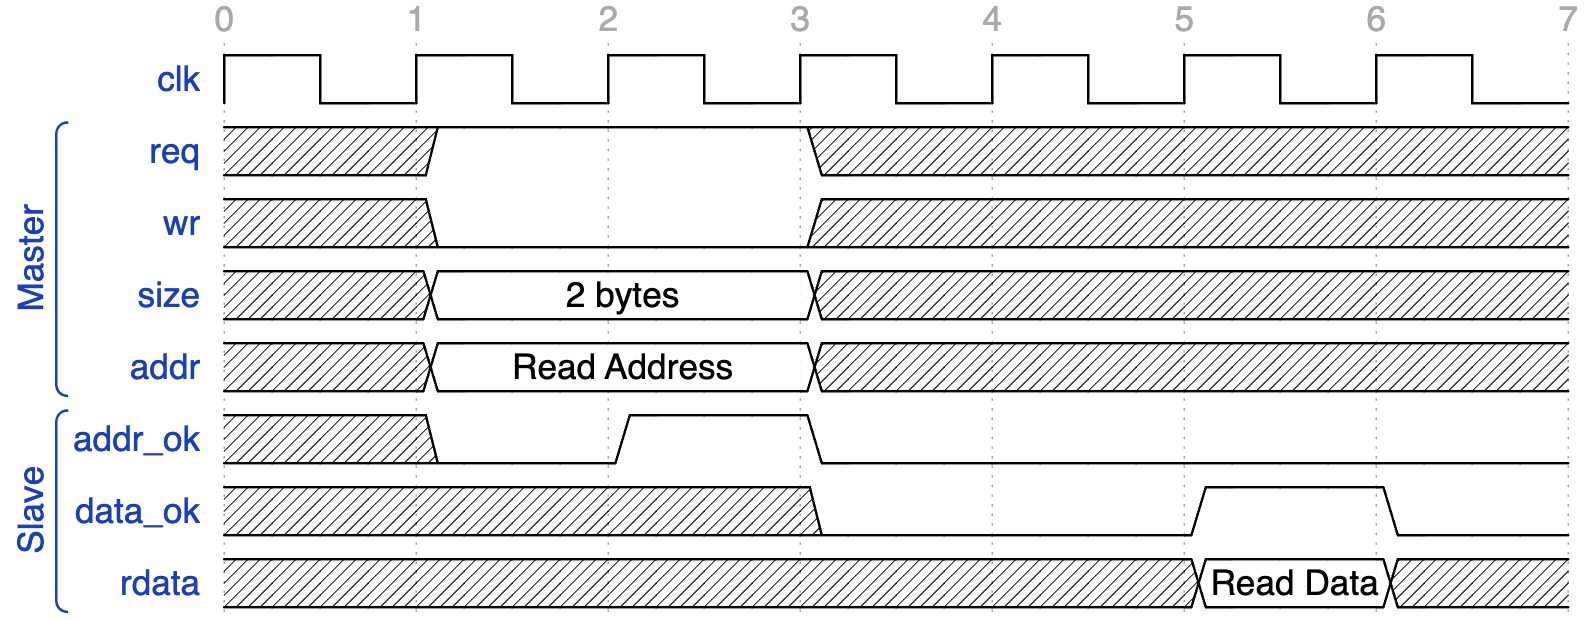
\includegraphics[width=1\linewidth]{assets/08/sram_read.jpg}
  \caption{类SRAM总线读事务时序图}
  \label{fig:sram-read}
\end{figure}

一次读事务可以被分解为几个关键步骤，每个步骤都发生在特定的时钟上升沿。

首先，在第一个时钟上升沿，主设备准备发起一个读请求。它通过设置请求信号\texttt{req}为高电平来通知从设备，同时将写请求信号\texttt{wr}保持在低电平，明确这是一个读操作而不是写操作。此时，主设备还会设置传输大小\texttt{size}为2 bytes，表明它希望读取两个字节的数据。

接着，在第二个时钟上升沿，主设备通过地址\texttt{addr}通道发送它想要读取的内存地址。这个地址被编码为特定的值，以便从设备能够识别和定位到正确的数据位置。此时，主设备和从设备尝试进行第一次握手。握手是通过地址确认信号\texttt{addr\_ok}来完成的。如果从设备成功接收并识别了地址，它会将\texttt{addr\_ok}信号设置为高电平，表示地址握手成功。然而，当前时刻握手失败了，所以在该时刻\texttt{addr\_ok}信号没有变为高电平，这可能是因为从设备需要额外的时间来准备或处理请求，无法单周期地接受请求数据。

到了第三个时钟上升沿，从设备准备好了，并通过将\texttt{addr\_ok}信号设置为高电平来确认地址握手成功。这意味着从设备已经接收并理解了主设备的请求，并且知道从哪个地址读取数据。

在接下来的两个时钟周期（第四和第五个时钟上升沿），主设备和从设备都在为数据传输做准备。主设备等待从设备将数据放到总线上，而从设备则在准备数据，以便在下一个时钟周期发送。在该过程中，从设备将数据握手信号\texttt{data\_ok}设置为低电平，即告知主设备读取请求仍在处理中，需要继续等待。

在第六个时钟上升沿，从设备完成了数据的读取，并通过读数据（\texttt{rdata}）信号将数据发送回主设备。同时，从设备设置数据确认信号（\texttt{data\_ok}）为高电平，表示数据握手成功，数据已经成功传输给主设备。

\subsubsection{写操作}\label{sec:08-bus-and-soc-007}

在类SRAM总线上进行一次写事务时的时序与读事务的类似。图\ref{fig:sram-write}展示了一个写操作的数据传输时序，与上面的读操作类似，但在时序细节上有所不同。

\begin{figure}[htbp]
  \centering
  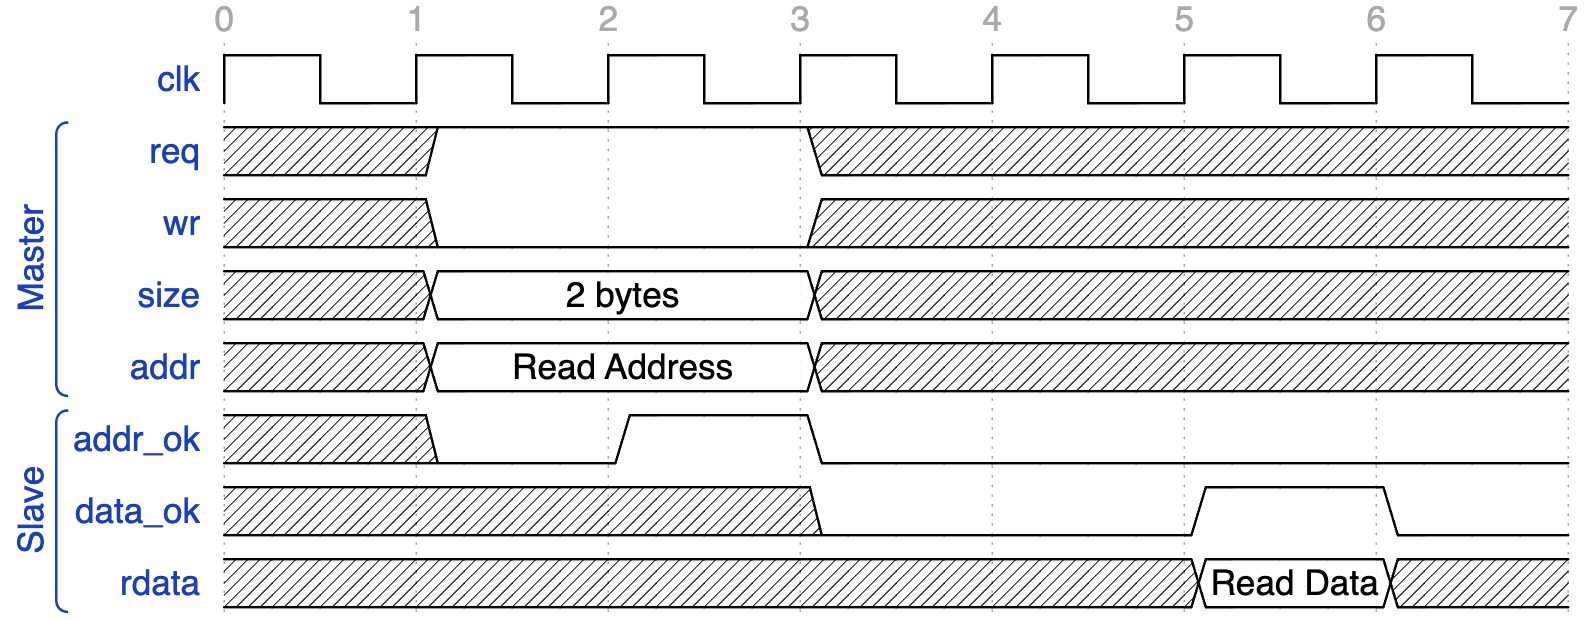
\includegraphics[width=1\linewidth]{assets/08/sram_write.jpg}
  \caption{类SRAM总线写事务时序图}
  \label{fig:sram-write}
\end{figure}

在第2个时钟上升沿，主端已设置好了写入的字节数\texttt{size}，写入地址\texttt{addr}和写入数据\texttt{wdata}，并将\texttt{wr}置高表示该事务为写事务，同时使用\texttt{req}通道向从方发送请求。

与上面读事务的时序图不同的是，在第2个时钟上升沿时，从方的\texttt{addr\_ok}直接为高电平，表示从方在单周期内成功接收了主方发送的所有数据信息。开发人员可以暂不关心从方具体是如何实现的，只需知道从方也可单周期接收数据，并在\texttt{req}置高的同时返回\texttt{addr\_ok}的握手信号。

在第二个时钟上升沿握手成功后，从方立即将\texttt{data\_ok}设置为低电平，告知主设备写入操作仍未完成。在等待三个周期后，在第6个时钟上升沿，\texttt{data\_ok}信号生效，从设备告知主设备写入完成。

至此，一次写操作结束。

\subsection{类SRAM总线的设计}\label{sec:08-bus-and-soc-008}

在类SRAM总线设计中，信号之间的约束关系直接影响总线的正确性和时序表现。以下是常见的约束和注意点：

\begin{itemize}
\tightlist
\item
  时序约束： \texttt{addr\_ok} 信号必须先于 \texttt{data\_ok} 激活，确保地址阶段先于数据阶段。
\item
  设计注意事项： 保持 \texttt{clk} 的稳定性是保证总线时序正确的基础；在高频率设计中，应特别关注信号传播延迟。
\end{itemize}

有些类SRAM总线协议包含特定要求。

作为开发者，在开发涉及类SRAM总线接口的功能时，需要仔细考虑这些信号的时序关系和协调。在发现总线相关的错误时，应当首先分析总线上握手信号和相关控制信号的波形，将主、从设备视为黑盒，分析是哪个设备执行出错，之后再进入下一个层次进行分析。尽量不要不区分层次地分析波形信号，因为在复杂CPU设计中信号层次很多，容易导致混乱。

在CPU设计中，类SRAM的各个控制信号的设计应根据具体的功能需求来优化：

\begin{itemize}
\tightlist
\item
  在取指令阶段，\texttt{addr\_ok} 的设计应确保地址信号能够在规定的时钟周期内传递到位，从而减少握手延迟。
\item
  在访存阶段 \texttt{data\_ok} 信号的设计应当灵活，以适应不同的数据大小传输需求。
\item
  优化时可使用流水线优化来提高数据吞吐量。
\item
  针对信号冲突，设计有效的仲裁机制，确保多主设备不会发生争用冲突。
\end{itemize}

\section{AXI总线协议}\label{sec:08-bus-and-soc-009}

AXI（Advanced eXtensible Interface）是一种广泛应用于现代片上系统（SoC）设计中的总线协议，它通过五个独立的通道实现主从设备之间的高效数据传输。每个通道可以独立工作，同时并发处理多个事务，这使得 AXI 总线在性能和灵活性上具有显著优势。

\subsection{接口信号}\label{sec:08-bus-and-soc-010}

AXI 协议将所有信号根据功能分为了五组，每组信号称为一个 \emph{通道}：读地址通道（Read Address Channel，AR），读数据通道（Read Data Channel，R），写地址通道（Write Address Channel，AW），写数据通道（Write Data Channel，W）以及写响应通道（Write Response Channel，B）。这五个通道负责处理从主设备到从设备的请求与响应过程，每个通道都有独特的信号集。

图\ref{fig:axi-channels}展示了AXI接口中的五个通道。读地址通道AR用于将主方希望读取的地址传输给从方，而从方读取到的数据将通过读数据通道R返回给主方。对于写操作，主方将写入地址及写入数据分别通过写地址通道AW和写数据通道W传输给从方，从方使用写响应通道B将是否正确写入的信息传输给主方。

\begin{figure}[htbp]
  \centering
  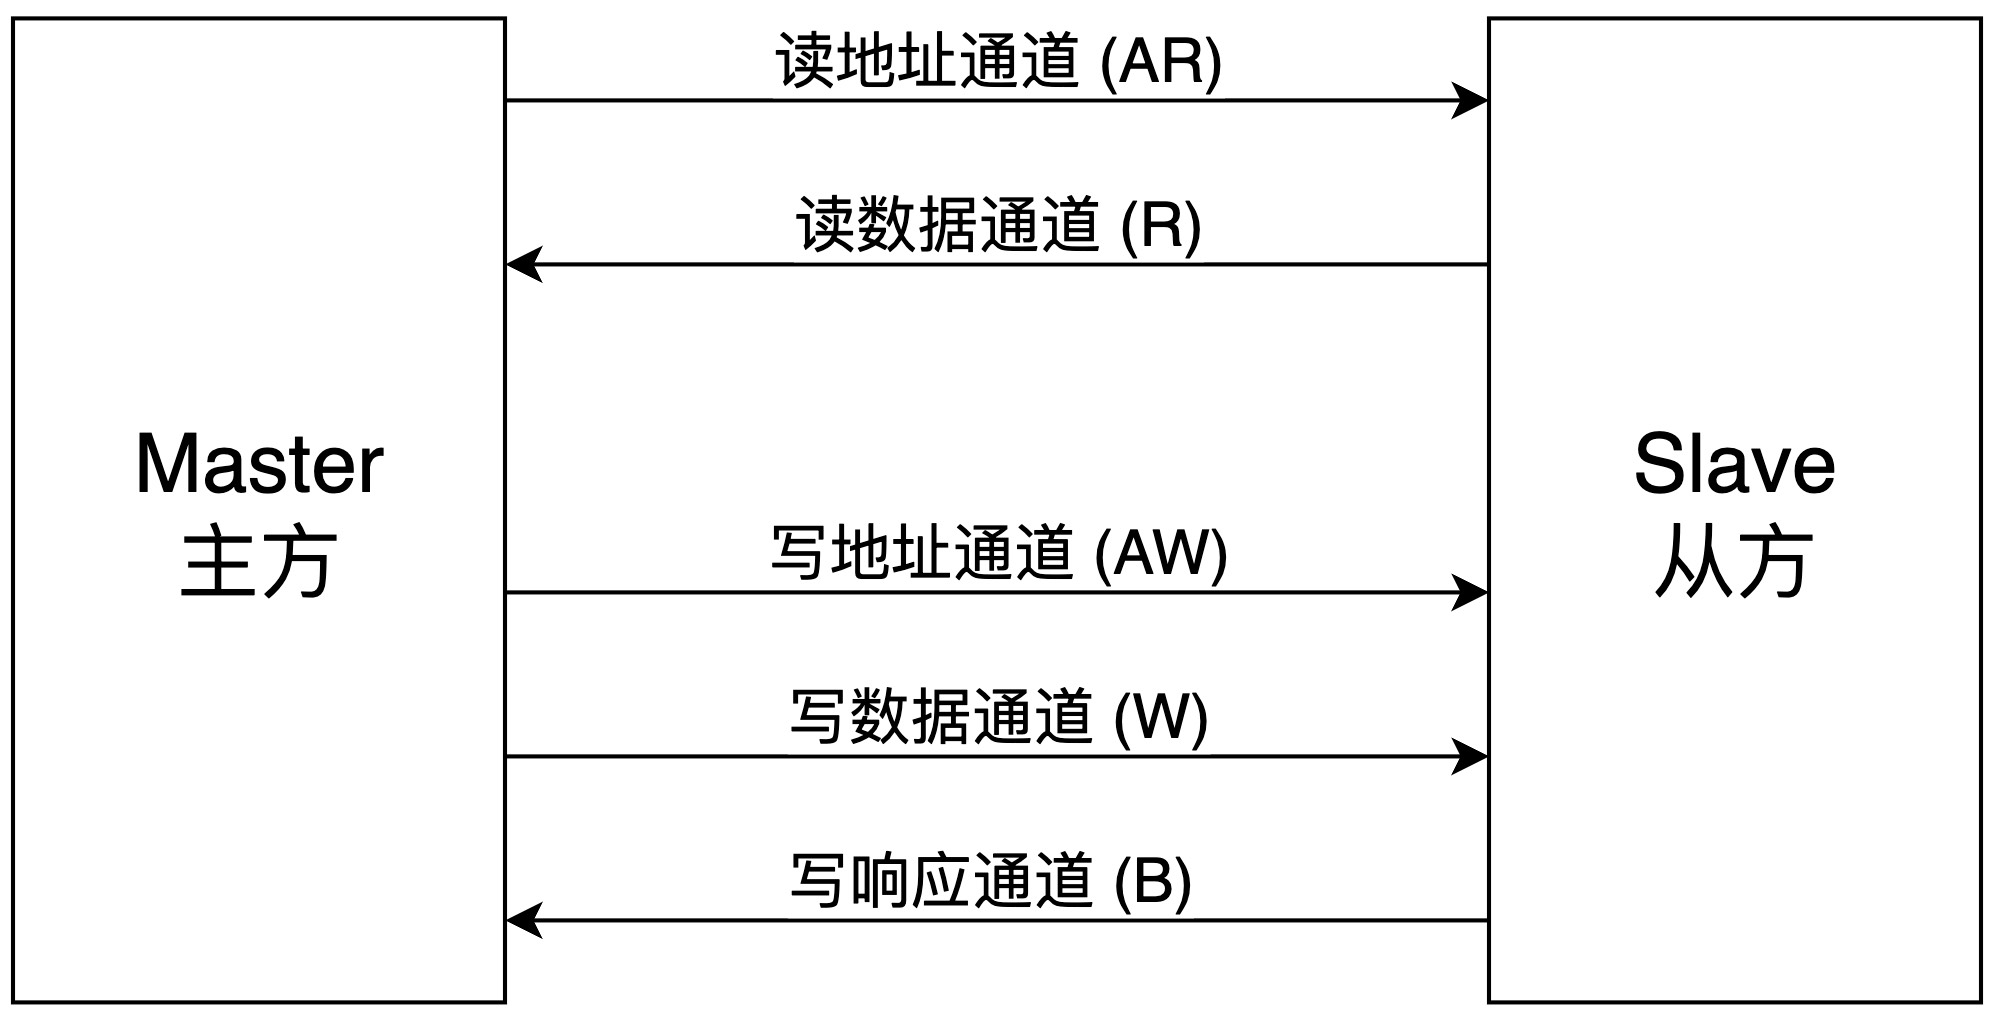
\includegraphics[width=0.7\linewidth]{assets/08/axi_channels.jpg}
  \caption{AXI总线通道示意图}
  \label{fig:axi-channels}
\end{figure}

应当注意的是，该图中的箭头方向指的是\textbf{数据流动的方向}，而并不直接表示信号的输入输出方向。每个通道内，均有从主方到从方以及从从方到主方的信号线路。例如，读地址通道用于将主方希望读取的地址通知从方，但从方也需要通过一些控制信号告知主方，主方传递的地址已收到，因此在该通道内仍需要由从方到主方的信号。这种用于确认对方是否正确接收好数据的信号称为 \emph{握手信号}，下面的某些小节将详细介绍AXI总线中的握手方法。

\subsubsection{读地址通道 (AR)}\label{sec:08-bus-and-soc-011}

\begin{longtable}[]{@{}
  >{\raggedright\arraybackslash}p{(\linewidth - 6\tabcolsep) * \real{0.1412}}
  >{\raggedright\arraybackslash}p{(\linewidth - 6\tabcolsep) * \real{0.1294}}
  >{\raggedright\arraybackslash}p{(\linewidth - 6\tabcolsep) * \real{0.2235}}
  >{\raggedright\arraybackslash}p{(\linewidth - 6\tabcolsep) * \real{0.5059}}@{}}
\toprule\noalign{}
\begin{minipage}[b]{\linewidth}\raggedright
信号
\end{minipage} & \begin{minipage}[b]{\linewidth}\raggedright
位宽
\end{minipage} & \begin{minipage}[b]{\linewidth}\raggedright
方向
\end{minipage} & \begin{minipage}[b]{\linewidth}\raggedright
功能
\end{minipage} \\
\midrule\noalign{}
\endhead
\bottomrule\noalign{}
\endlastfoot
ARID & 4-16 bits & Master → Slave & 传输读请求的标识符，用于区分不同的事务 \\
ARADDR & 32-64 bits & Master → Slave & 传输读地址，指示从何处读取数据 \\
ARLEN & 4 bits & Master → Slave & 传输突发传输的长度，指示读取多少个数据字 \\
ARSIZE & 3 bits & Master → Slave & 传输数据的大小，表示每个传输的数据字节数 \\
ARBURST & 2 bits & Master → Slave & 传输突发传输类型，支持递增、包装和固定 \\
ARVALID & 1 bit & Master → Slave & 表示读地址有效，启动握手 \\
ARREADY & 1 bit & Slave → Master & 表示从设备已准备好接收读地址 \\
\end{longtable}

\textbf{重点信号说明：}

\begin{itemize}
\item
  \textbf{ARID}：用于区分主设备发起的多个并发读请求。每个请求的 ARID 唯一标识该请求。
\item
  \textbf{ARADDR}：传输内存地址，主设备发出读请求时，需要指定从哪个地址读取数据。
\item
  \textbf{ARVALID 与 ARREADY}：ARVALID 表示主设备的地址和控制信号有效，而 ARREADY 则是从设备的响应信号，当二者同时为高时，地址握手完成。
\end{itemize}

\subsubsection{读数据通道 (R)}\label{sec:08-bus-and-soc-012}

\begin{longtable}[]{@{}
  >{\raggedright\arraybackslash}p{(\linewidth - 6\tabcolsep) * \real{0.1412}}
  >{\raggedright\arraybackslash}p{(\linewidth - 6\tabcolsep) * \real{0.1294}}
  >{\raggedright\arraybackslash}p{(\linewidth - 6\tabcolsep) * \real{0.2235}}
  >{\raggedright\arraybackslash}p{(\linewidth - 6\tabcolsep) * \real{0.5059}}@{}}
\toprule\noalign{}
\begin{minipage}[b]{\linewidth}\raggedright
信号
\end{minipage} & \begin{minipage}[b]{\linewidth}\raggedright
位宽
\end{minipage} & \begin{minipage}[b]{\linewidth}\raggedright
方向
\end{minipage} & \begin{minipage}[b]{\linewidth}\raggedright
功能
\end{minipage} \\
\midrule\noalign{}
\endhead
\bottomrule\noalign{}
\endlastfoot
RID & 4-16 bits & Slave → Master & 传输读请求的标识符，表示正在返回哪个事务的数据 \\
RDATA & 32-64 bits & Slave → Master & 传输读到的数据 \\
RRESP & 2 bits & Slave → Master & 传输读数据的响应状态（OKAY、ERROR等） \\
RLAST & 1 bit & Slave → Master & 表示这是突发传输的最后一个数据字 \\
RVALID & 1 bit & Slave → Master & 表示读数据有效，启动握手 \\
RREADY & 1 bit & Master → Slave & 表示主设备已准备好接收读数据 \\
\end{longtable}

\textbf{重点信号说明：}

\begin{itemize}
\item
  \textbf{RDATA}：主设备从从设备读取的数据，通过该信号传递给主设备。
\item
  \textbf{RLAST}：当进行突发传输时，RLAST 表示突发传输的最后一个数据字。
\item
  \textbf{RVALID 与 RREADY}：当 RVALID 为高时，表示从设备传输的数据有效；RREADY 为高时，表示主设备准备好接收数据。
\end{itemize}

\subsubsection{写地址通道 (AW)}\label{sec:08-bus-and-soc-013}

\begin{longtable}[]{@{}
  >{\raggedright\arraybackslash}p{(\linewidth - 6\tabcolsep) * \real{0.1412}}
  >{\raggedright\arraybackslash}p{(\linewidth - 6\tabcolsep) * \real{0.1294}}
  >{\raggedright\arraybackslash}p{(\linewidth - 6\tabcolsep) * \real{0.2235}}
  >{\raggedright\arraybackslash}p{(\linewidth - 6\tabcolsep) * \real{0.5059}}@{}}
\toprule\noalign{}
\begin{minipage}[b]{\linewidth}\raggedright
信号
\end{minipage} & \begin{minipage}[b]{\linewidth}\raggedright
位宽
\end{minipage} & \begin{minipage}[b]{\linewidth}\raggedright
方向
\end{minipage} & \begin{minipage}[b]{\linewidth}\raggedright
功能
\end{minipage} \\
\midrule\noalign{}
\endhead
\bottomrule\noalign{}
\endlastfoot
AWID & 4-16 bits & Master → Slave & 传输写请求的标识符 \\
AWADDR & 32-64 bits & Master → Slave & 传输写地址，指示将数据写入哪个地址 \\
AWLEN & 4 bits & Master → Slave & 传输突发传输的长度 \\
AWSIZE & 3 bits & Master → Slave & 传输数据大小，表示每次传输的数据字节数 \\
AWBURST & 2 bits & Master → Slave & 传输突发类型（递增、包装或固定） \\
AWVALID & 1 bit & Master → Slave & 表示写地址有效，启动握手 \\
AWREADY & 1 bit & Slave → Master & 表示从设备已准备好接收写地址 \\
\end{longtable}

\textbf{重点信号说明：}

\begin{itemize}
\item
  \textbf{AWADDR}：与读地址通道类似，AWADDR 传输写地址，指定要写入的内存地址。
\item
  \textbf{AWLEN}：指示突发传输的总长度，即一次写操作要写入的总数据字个数。
\item
  \textbf{AWVALID 与 AWREADY}：类似于读通道的握手信号，AWVALID 表示写地址有效，AWREADY 则表示从设备准备好接收写地址。
\end{itemize}

\subsubsection{写数据通道 (W)}\label{sec:08-bus-and-soc-014}

\begin{longtable}[]{@{}
  >{\raggedright\arraybackslash}p{(\linewidth - 6\tabcolsep) * \real{0.1412}}
  >{\raggedright\arraybackslash}p{(\linewidth - 6\tabcolsep) * \real{0.1294}}
  >{\raggedright\arraybackslash}p{(\linewidth - 6\tabcolsep) * \real{0.2235}}
  >{\raggedright\arraybackslash}p{(\linewidth - 6\tabcolsep) * \real{0.5059}}@{}}
\toprule\noalign{}
\begin{minipage}[b]{\linewidth}\raggedright
信号
\end{minipage} & \begin{minipage}[b]{\linewidth}\raggedright
位宽
\end{minipage} & \begin{minipage}[b]{\linewidth}\raggedright
方向
\end{minipage} & \begin{minipage}[b]{\linewidth}\raggedright
功能
\end{minipage} \\
\midrule\noalign{}
\endhead
\bottomrule\noalign{}
\endlastfoot
WDATA & 32-64 bits & Master → Slave & 传输要写入的数据 \\
WSTRB & 4-8 bits & Master → Slave & 数据写入时的字节掩码，指示哪些字节有效 \\
WLAST & 1 bit & Master → Slave & 表示突发传输中的最后一个数据字 \\
WVALID & 1 bit & Master → Slave & 表示写数据有效，启动握手 \\
WREADY & 1 bit & Slave → Master & 表示从设备已准备好接收写数据 \\
\end{longtable}

\textbf{重点信号说明：}

\begin{itemize}
\item
  \textbf{WDATA}：主设备要写入从设备的数据通过该信号传递。
\item
  \textbf{WSTRB}：写数据时的字节掩码，用于指示哪些字节有效，这在非对齐或部分写操作中尤为重要。
\item
  \textbf{WLAST}：当进行突发传输时，WLAST 信号用于指示写数据的最后一个数据字。
\end{itemize}

\subsubsection{写响应通道 (B)}\label{sec:08-bus-and-soc-015}

\begin{longtable}[]{@{}
  >{\raggedright\arraybackslash}p{(\linewidth - 6\tabcolsep) * \real{0.1412}}
  >{\raggedright\arraybackslash}p{(\linewidth - 6\tabcolsep) * \real{0.1294}}
  >{\raggedright\arraybackslash}p{(\linewidth - 6\tabcolsep) * \real{0.2235}}
  >{\raggedright\arraybackslash}p{(\linewidth - 6\tabcolsep) * \real{0.5059}}@{}}
\toprule\noalign{}
\begin{minipage}[b]{\linewidth}\raggedright
信号
\end{minipage} & \begin{minipage}[b]{\linewidth}\raggedright
位宽
\end{minipage} & \begin{minipage}[b]{\linewidth}\raggedright
方向
\end{minipage} & \begin{minipage}[b]{\linewidth}\raggedright
功能
\end{minipage} \\
\midrule\noalign{}
\endhead
\bottomrule\noalign{}
\endlastfoot
BID & 4-16 bits & Slave → Master & 传输写事务的标识符 \\
BRESP & 2 bits & Slave → Master & 传输写操作的响应状态 \\
BVALID & 1 bit & Slave → Master & 表示写响应有效，启动握手 \\
BREADY & 1 bit & Master → Slave & 表示主设备已准备好接收写响应 \\
\end{longtable}

\textbf{重点信号说明：}

\begin{itemize}
\item
  \textbf{BRESP}：传输写操作的结果状态（如 OKAY、ERROR），用于指示写操作是否成功完成。
\item
  \textbf{BVALID 与 BREADY}：BVALID 表示从设备传输的响应有效，BREADY 则表示主设备已准备好接收响应。
\end{itemize}

\subsection{握手机制}\label{sec:08-bus-and-soc-016}

在每个通道内，AXI均设计了一对握手信号，即\texttt{VALID}和\texttt{READY}。在不同的通道中，这些握手信号将以通道名+\texttt{VALID}或\texttt{READY}的形式命名。因此，AXI总线共含有5对握手信号。例如，在B通道内，握手信号的名称为\texttt{BVALID}和\texttt{BREADY}。

AXI 的握手机制就通过每个通道内的握手信号完成。每个通道是独立的一组信息传递单元，每个通道内的握手信号控制了该通道内所有数据的传输。AXI总线上复杂的信息传输，是通过五个通道内的信息传输所构成的。

握手机制的关键在于，只有当该通道的 \texttt{VALID} 和 \texttt{READY} 信号都为高时，数据传输才会发生。
例如，图\ref{fig:axi-handshake}展示了读地址通道的握手时序。

\begin{figure}[htbp]
  \centering
  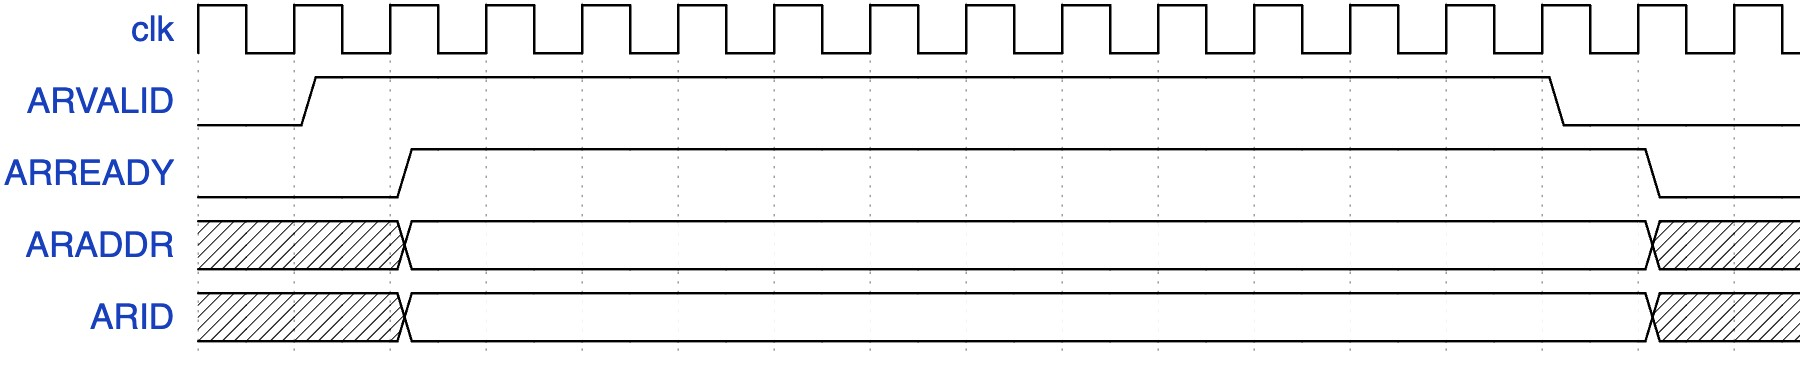
\includegraphics[width=1\linewidth]{assets/08/axi_handshake.jpg}
  \caption{AXI总线AR端口握手信号时序图}
  \label{fig:axi-handshake}
\end{figure}

在时钟上升沿时，如果 ARVALID 和 ARREADY 同时为高，表示主从设备之间的握手完成，地址传输成功。

\subsection{总线事务}\label{sec:08-bus-and-soc-017}

AXI总线事务通常由多个握手过程组合完成。读事务和写事务分别通过不同的通道进行通信。

\subsubsection{读事务}\label{sec:08-bus-and-soc-018}

完整的读事务包括一次读地址通道的握手和一次读数据通道的握手。在读事务开始时，主设备通过 AR 通道传输地址信息，随后从设备在 R 通道上返回数据。在AR通道内和R通道内的数据传输中，分别需要一次握手，即\texttt{VALID}和\texttt{READY}信号同时生效时产生的数据传输。

图\ref{fig:axi-read}展示了AXI总线的一次读事务的完整过程，其中有些信号被省略。

\begin{figure}[htbp]
  \centering
  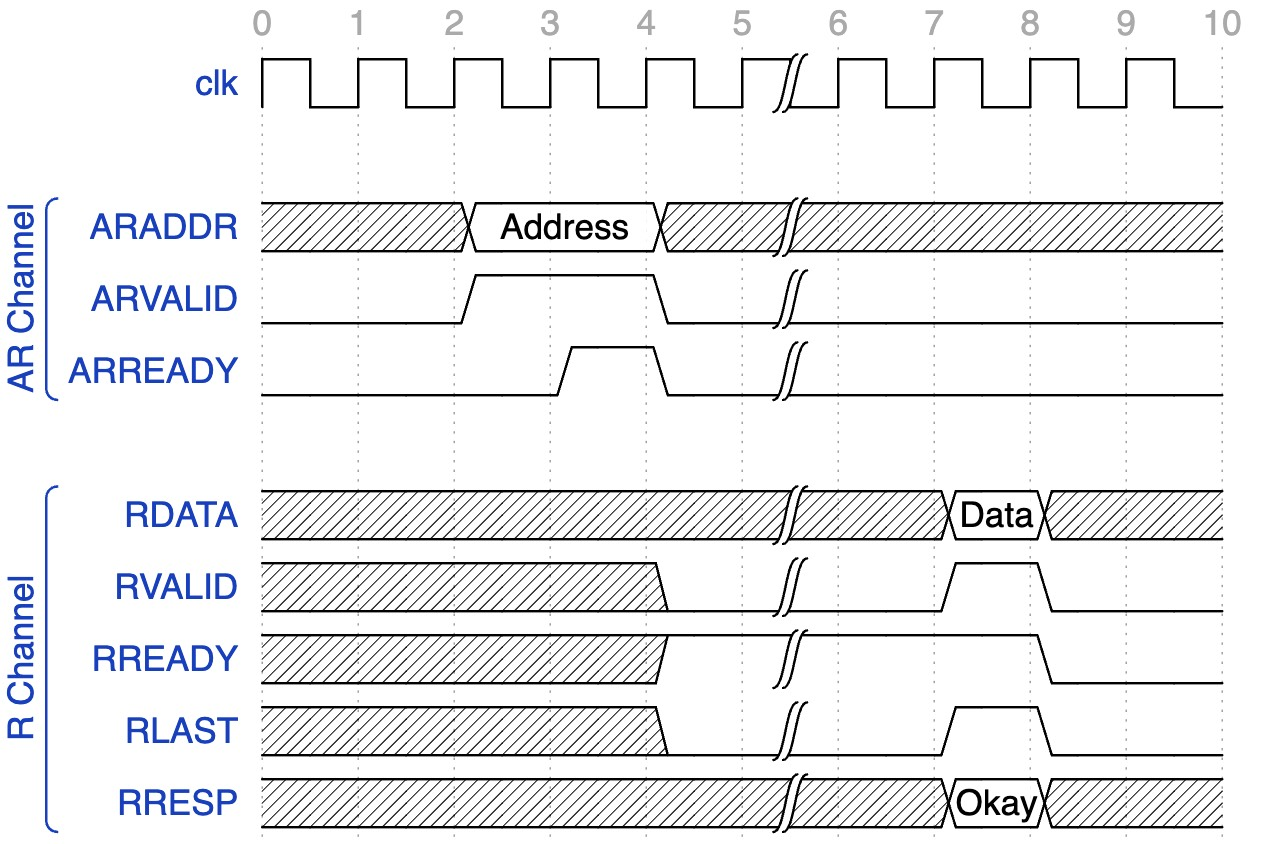
\includegraphics[width=1\linewidth]{assets/08/axi_read.jpg}
  \caption{AXI总线读事务时序图}
  \label{fig:axi-read}
\end{figure}

在上述时序图中，第2个时钟上升沿之后，ARVALID 生效，表示主设备已通过ARADDR通道准备好发送读地址。
在第3个时钟上升沿时，ARREADY为低电平，表示从设备没有准备好接收，于是主设备继续维持ARADDR不变，并持续将ARVALID置高。

在第4个时钟上升沿时，ARREADY被从方置高。此时，ARVALID和ARREADY同时生效，说明AR通道握手成功，即从设备已经接受了ARADDR信号表示的读地址，以及其他一些读取设置参数（这些信号在本图中被省略）。

下面，从设备应当通过R通道，向主设备发送读取到的数据。由于从设备在接受好读地址之后，可能需要一定的时间才能成功获取数据，因此RVALID将首先被从方设置为低电平。同时，由于主方已经做好了接受数据的准备，因此它将RREADY在第5个时钟上升沿置高。实际情况中，主方有可能并不会在AR通道握手成功后，立刻将RREADY置高，因为可能需要一定时间才能完成接受数据的准备。

在之后的一段时间内，主设备等待从设备进行数据的读取。

在图中的第8个时钟上升沿时，从设备将读取数据准备好，并将RDATA数据设置为正确的值。与此同时，将RVALID置高。
此时，R通道成功握手。
在此图中RLAST信号也为高，说明该数据是本组传输的最后一个数据。
在突发传输模式中，该信号具有重要的用途。后文将详细介绍。

\subsubsection{写事务}\label{sec:08-bus-and-soc-019}

写事务包括三次握手，分别为写地址（AW）、写数据（W）、写响应（B）通道的握手。主设备先通过 AW 通道传输写地址，随后通过 W 通道传输写数据，最后从设备通过 B 通道返回写操作的响应。在整个过程中，需要三次握手，分别对应三个通道的数据传输。

图\ref{fig:axi-write}展示了AXI总线的一次写事务的完整过程，其中有些信号被省略。

\begin{figure}[htbp]
  \centering
  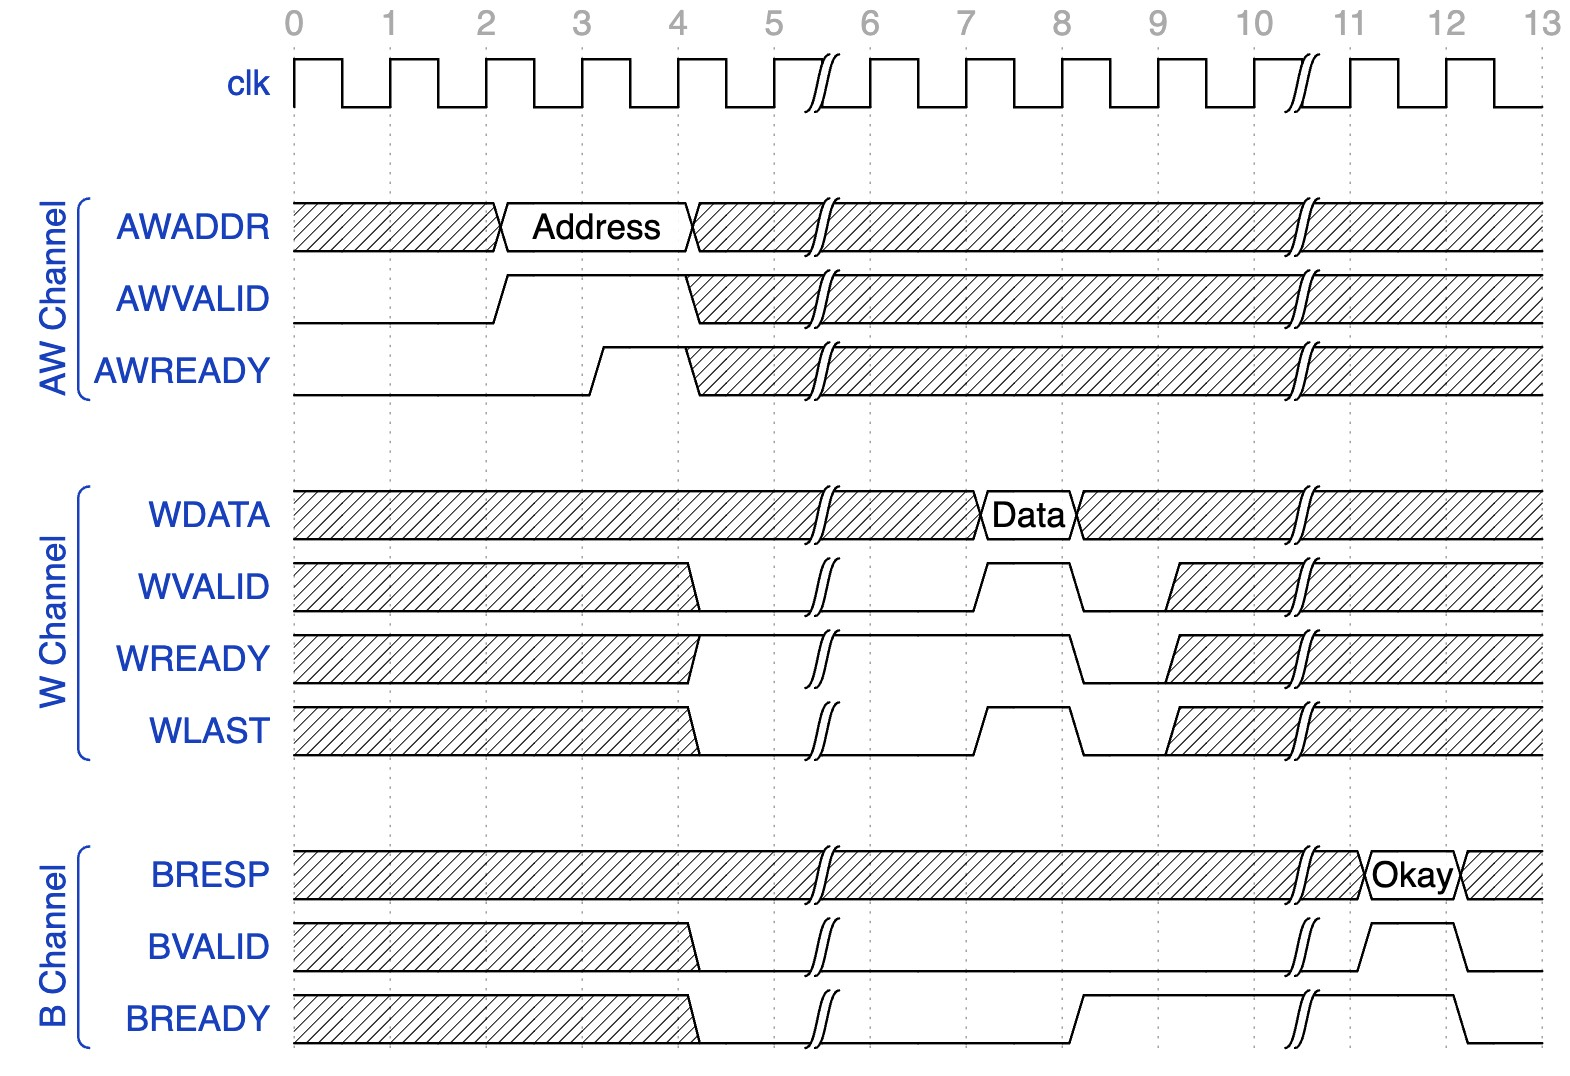
\includegraphics[width=1\linewidth]{assets/08/axi_write.jpg}
  \caption{AXI总线写事务时序图}
  \label{fig:axi-write}
\end{figure}

从图中可以看出，总共有AW、W、B三个通道参与了信息传递。

在前5个时钟周期，AW通道进行了地址的传输，告知了从方待写入的地址。具体的握手过程与上小节介绍的在读事务中AR通道进行的地址传输基本相同。在第4个时钟上升沿，完成了握手。

之后，主方将通过W通道，将待写入的数据发送给从方。从方先将WREADY设置为1，表示从方已做好准备接受写入的数据。然而，此时主方并没有准备好数据，因此WVALID一直为0，此时从方需要等待。在第8个时钟上升沿，WVALID为高，表示数据已经在WDATA信号中准备好。同时WLAST为1，表示该数据为本组传输中最后一个数据（其他使用方法见突发传输一节）。至此，从方已经接受了主方发送的全部信息，包括待写入的地址和数据。在本图中忽略的其他信号中，主方还进行了写入字节数等设置。

此时从方可以开始完成数据的写入工作，并且需要在写入完成后，将写入结果通过B通道发送给主方，告知是否写入成功。在写入正在进行时，从方将BVALID设置为0，而BREADY由主方设置为1，表明主方时刻做好了接受写入结果信息的准备，但从方仍在进行写入工作，或者写入工作进行完成但没有准备好结果信息的数据。在其他的情况中，可能BREADY会被置为0，这表明主方没有做好接受写入结果信息的准备。本图只表示所有可能情况中的一种，开发人员需要根据具体情况进行分析。

在第12个时钟上升沿，从方将Okay消息传输给从方，并在B通道成功握手。此时，一次写事务成功完成。从方也可能会将错误信息通过B通道传递给主方，表示写入失败，这种情况下主方需要进行一些错误处理，例如重传。

\subsection{突发传输模式}\label{sec:08-bus-and-soc-020}

在AXI总线中，\textbf{突发传输模式（burst mode）}是一种能够提高数据传输效率的方式。突发传输允许主设备（Master）发出一次地址请求，随后从设备（Slave）在不需要额外地址请求的情况下，连续传输多个数据。这样可以减少每次传输地址带来的延迟，大幅提高数据带宽，特别适合缓存、内存等连续读写场景。

\subsubsection{突发传输类型}\label{sec:08-bus-and-soc-021}

AXI协议支持三种不同的突发传输类型：

\begin{enumerate}
\def\labelenumi{\arabic{enumi}.}
\item
  \textbf{固定突发（Fixed Burst）}：所有传输使用相同的地址。适用于外设寄存器读取等场景。
\item
  \textbf{增量突发（Incrementing Burst）}：每次传输地址递增，适合连续存储器读取操作。地址按照数据位宽自动递增，例如每次传输32位数据时，地址增量为4字节。
\item
  \textbf{环形突发（Wrapping Burst）}：在传输过程中，当达到指定的最大地址时，地址将回绕到起始地址。常用于支持关键字优先的缓存操作，即在一个cache行中，先读取当前CPU流水线所需要的数据，并且立即返回给CPU流水线，在流水线继续工作的同时，再继续读取该cache行中其他位置的数据并存入cache中。AXI的环形突发模式可以很完美的适配于关键字优先技术。
\end{enumerate}

突发传输的长度可以是1到256个数据拍（beat）。主设备通过 ARLEN 或 AWLEN 信号指定传输的长度。

\subsubsection{突发传输的时序}\label{sec:08-bus-and-soc-022}

\begin{figure}[htbp]
  \centering
  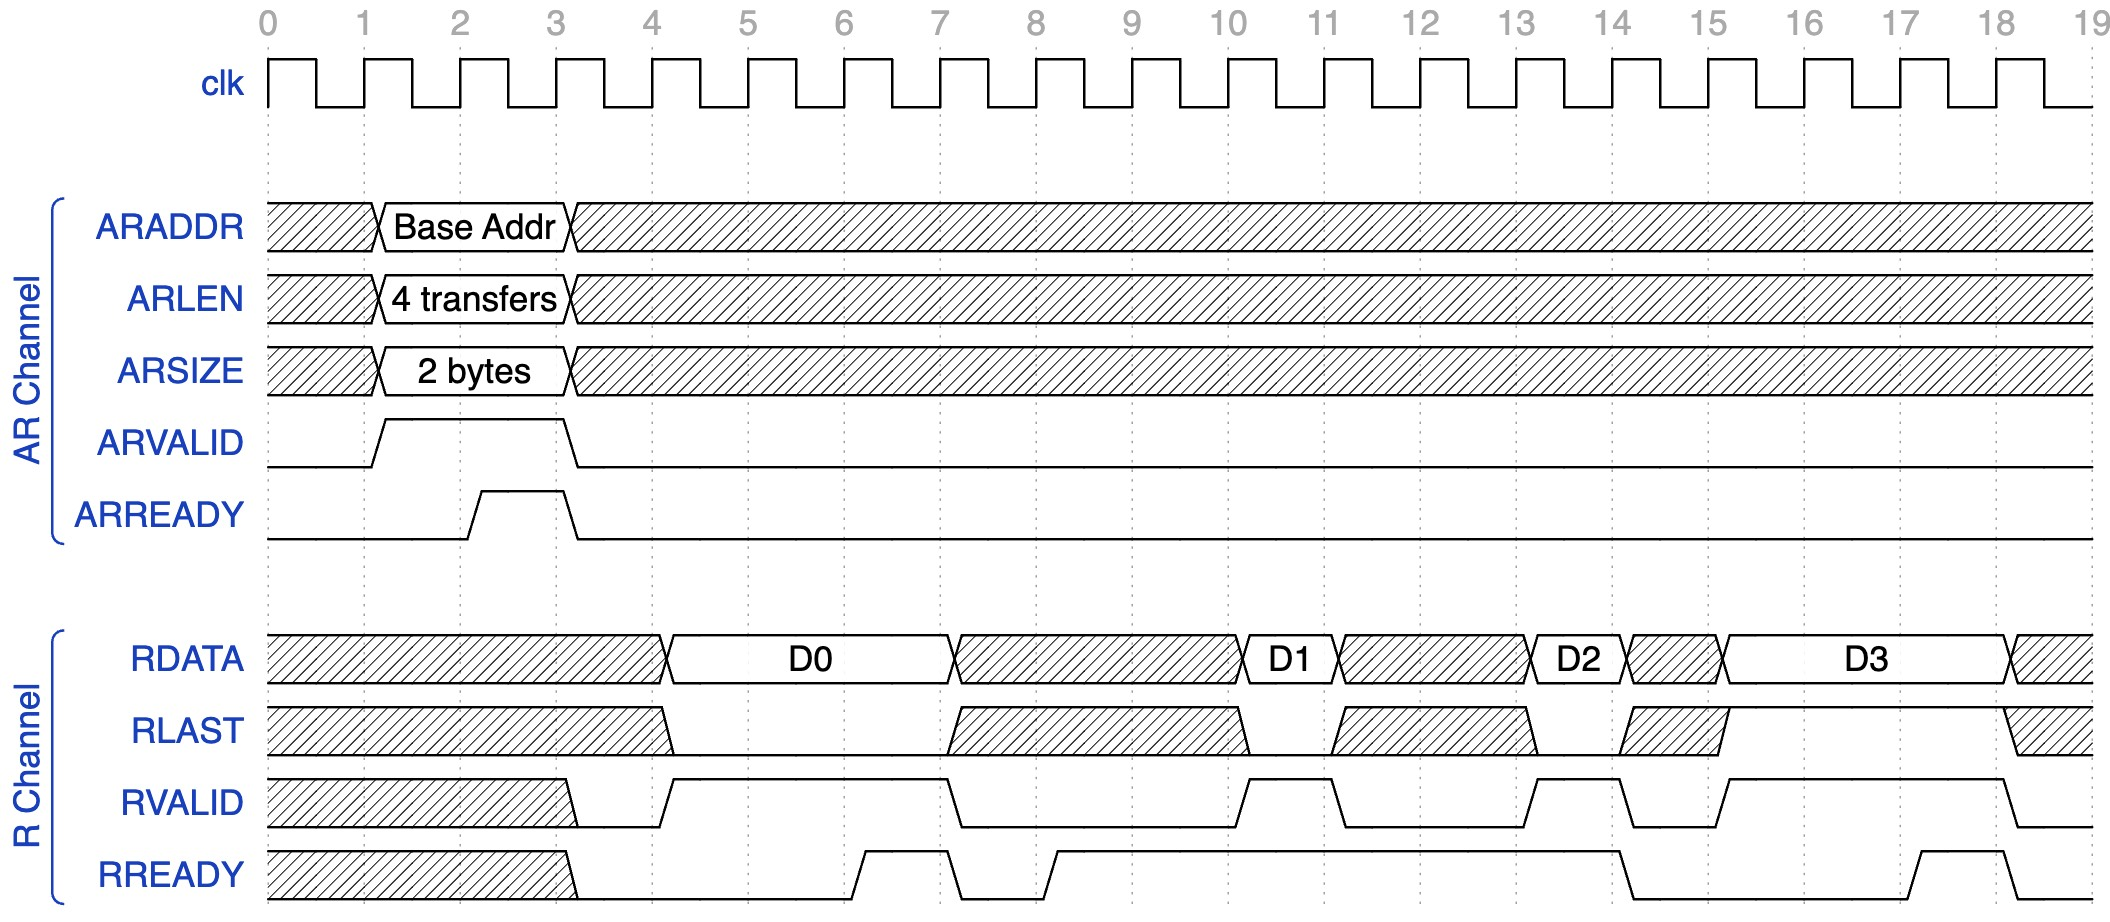
\includegraphics[width=1\linewidth]{assets/08/axi_burst.jpg}
  \caption{AXI总线突发传输读事务时序图}
  \label{fig:axi-burst}
\end{figure}

图\ref{fig:axi-burst}展示了AXI总线的突发传输模式中，一次读事务的时序图。

突发传输模式是在主方通过AR通道发送读请求，或者通过AW通道发送写请求时，通过\texttt{ARLEN/AWLEN}和\texttt{ARBURST/AWBURST}设置的。\texttt{ARLEN/AWLEN}设置了本次读/写事务中的数据传输次数，在本图中主方设置为了4，表示在本次读事务中需要连续传输4次数据。\texttt{ARBURST/AWBURST}设置了本次读/写事务的类型，包括上小节提到的三种，该信号在本图中被省略，从方将根据该配置信息决定在本次的读/写事务中，每次发送/接受的数据地址该如何变化（例如全部使用相同地址、地址递增、或者环形增加）。

在图中的第3个时钟上升沿，AR通道完成了握手。\texttt{ARSIZE}设置的是一次数据传输将传输2字节的数据，\texttt{ARADDR}设置了本次突发传输的基地址。因此，从方将通过R通道向主方发送以\texttt{ARADDR}地址为首地址的数据，每次数据传输将发送2字节数据，总共含有4次数据传输。因此，在本次读事务中将读取共8字节的数据。

在每次只能最多传输2字节的情况下，若不使用突发传输，传输共8字节的数据需要主方发起4次读事务，这表示主方需要通过AR通道发送4次地址信息，而从方需要通过R通道发送4次数据信息。在本图所示的突发传输模式下，主方只需要通过AR通道发送1次地址信息，同时进行突发传输模式配置，之后从方可连续地通过R通道发送4次数据信息，减少了AR通道的3次握手。由于一次读取的数据块更大，因此从方设备可能也能更快的作出响应，提高了总线效率。

在第4到第7个时钟上升沿中，从方通过R通道发送了第一个数据\(D0\)，并将RVALID置高，同时将RLAST置低。RLAST信号表示当前发送的数据是否为本此读事务的最后一次数据传输。本次读事务总共需要完成4次数据传输，因此此时传输的第一个数据不是最后一次数据传输，因此RLAST为0。由于一开始主方并未做好接受准备，因此RREADY在4-6个时钟上升沿时都为0，并在第7个时钟上升沿成功握手。

在第9个时钟上升沿，主方设备做好了接受准备，但从方并没有完成数据的读取，因此RVALID为低但RREADY为高，主方等待从方传输数据。在第11个时钟上升沿，第二个数据\(D1\)成功握手，RLAST也为0。同理，在第14个时钟上升沿，完成了第三个数据传输。

从第16个时钟上升沿开始，从方开始在RDATA发送最后一组数据\(D3\)，同时将RLAST置高，告知主方在本次数据传输结束后，本次读事务将结束。在第18个时钟上升沿时成功握手，标志着最后一组数据的成功传输，以及本次读事务的结束。

\subsubsection{突发传输的应用和实现}\label{sec:08-bus-and-soc-023}

突发传输特别适合缓存设计。例如，处理器从主内存读取数据时，通常以块的形式读取多个连续地址的内容。突发模式允许一次性传输整个数据块，减少了多个单独请求的开销。突发传输的另一个应用场景是DMA（直接内存访问）操作。DMA传输通常涉及大量数据的连续传输，突发传输能够极大提高DMA通道的效率，减少系统总线的占用时间。

在CPU实现过程中，应尽量选择适合数据块大小的突发长度，以充分利用传输带宽。例如，对于缓存行大小为64字节的系统，可以选择传输8个32位的数据拍。另外，应尽量减少突发传输之间的间隔时间，确保数据连续传输，避免总线资源浪费。

\subsection{其他总线特性}\label{sec:08-bus-and-soc-024}

AXI 总线还具有其他显著的特性，例如并发访问、乱序响应和 ID 信号的使用。以下将详细介绍这些特性。

AXI 总线允许\textbf{并发访问}，这意味着不同的事务可以同时在多个通道中进行。主设备能够在多个通道中并发发起地址、数据和响应传输，而从设备则通过握手机制协调这些并发事务。例如，主设备可以在发起写事务的同时发起另一个读事务。AXI 总线的并发特性提高了数据传输的效率，使系统能够更好地利用带宽资源。

\textbf{乱序响应}是 AXI 总线的一大优势，它允许从设备以不同于请求顺序的方式响应主设备的请求。这种灵活性使得 AXI 总线在处理复杂的、多线程操作时表现出色。然而，乱序响应也带来了系统设计上的挑战，设计者需要确保主设备能够正确地管理这些乱序响应，避免数据的混淆。

AXI 总线中的 \textbf{ID 信号}为事务的识别提供了重要支持。每个事务可以携带一个唯一的 ID 标识符，用来区分不同事务或线程的请求。这对于处理多线程的并行操作非常有用，特别是在一个主设备发起多个请求时，ID 可以确保从设备能正确识别和响应每一个事务。

\section{类SRAM总线与AXI总线桥接设计}\label{sec:08-bus-and-soc-025}

在设计计算机系统时，类SRAM总线与AXI总线的桥接设计是非常重要的一环。它不仅能够确保两种不同总线系统之间的互操作性，还可以提高系统整体的性能和可靠性。类SRAM总线较为简洁，因此可以用作内部设计时的接口。而AXI性能较高，有多种高性能传输特性，功能全面，适合作为片上总线，连接SoC上的不同设备。因此，往往需要设计类SRAM总线与AXI总线的转接桥。
在桥接设计中，关键任务之一是将两种总线的接口信号正确映射和转换，保证它们之间的数据传输和控制流的正确进行。

\subsection{类SRAM总线接口信号和AXI总线接口信号的关系}\label{sec:08-bus-and-soc-026}

类SRAM总线通常用于片上系统，信号较为简洁。主要信号包括请求信号req，地址信号addr，数据握手信号addr\_ok和data\_ok，以及读/写数据信号。而AXI总线作为一种更复杂的总线协议，定义了多个通道，分别处理地址、数据和响应等信息。在AXI协议中，关键信号包括地址写通道AWVALID和AWREADY，数据写通道WVALID和WREADY，以及响应通道BVALID和BREADY。类似的读操作则有ARVALID、ARREADY（地址通道）和RVALID、RREADY（数据通道）信号。为了让类SRAM总线和AXI总线成功通信，必须通过转接桥进行信号的映射和转换。下面将讨论类SRAM信号与AXI信号的具体对应关系及转换策略。

\textbf{请求信号\texttt{req}与AXI的\texttt{AWVALID/ARVALID}}：在类SRAM总线中，req信号用于表示开始一次读或写操作。在AXI总线中，读和写操作被分成了不同的通道，分别使用AWVALID和ARVALID信号。因此，设计转接桥时，需要将req信号根据操作的类型映射为AWVALID（写操作）或ARVALID（读操作）。

\textbf{地址信号\texttt{addr}与AXI的\texttt{AWADDR/ARADDR}}：类SRAM中的addr信号用于指定内存地址。在AXI中，地址通道分为读地址通道（ARADDR）和写地址通道（AWADDR）。因此，addr信号可以直接映射到相应的AXI地址信号上，具体映射到哪一个通道取决于请求的类型（读或写）。

\textbf{握手信号\texttt{addr\_ok}和\texttt{data\_ok}与AXI的\texttt{READY/VALID}}：在类SRAM中，addr\_ok和data\_ok信号用于进行地址和数据阶段的握手。相应的，AXI总线使用VALID和READY信号进行类似的握手机制。例如，类SRAM的addr\_ok信号可以映射为AXI的AWREADY或ARREADY，而data\_ok则对应WREADY（写数据通道）或RREADY（读数据通道）。在设计转接桥时，需要确保这些握手信号在合适的时机进行转换，并且在VALID和READY信号同时为高时，触发数据传输。

\textbf{数据信号\texttt{rdata}与AXI\texttt{的RDATA}}：rdata信号在类SRAM中表示读取的数据，而AXI的RDATA信号则用于传输读取的数据。转接桥设计时，可以直接将rdata信号映射到AXI的RDATA通道。

\textbf{数据大小信号\texttt{size}与AXI的\texttt{ARSIZE/AWSIZE}}：类SRAM中的size信号用来指示传输数据的大小，而在AXI中，ARSIZE和AWSIZE信号也有类似功能，分别用于指定读和写操作的数据宽度。因此，类SRAM的size信号可以直接映射到AXI相应的信号上，转接桥需要确保数据宽度的一致性，避免传输错误。

\subsection{转接桥的顶层接口}\label{sec:08-bus-and-soc-027}

通常，转接桥的顶层接口包括指令段和数据段的类SRAM接口，以及AXI总线的RAM接口。指令段和数据段分别处理不同类型的数据请求，这种设计有助于减少请求之间的竞争，提高数据传输效率。

指令段的类SRAM接口用于处理与程序指令相关的存取请求。通常，这部分接口的设计要求较为简单，因为指令请求多为顺序访问，且数据量相对较小。相比之下，数据段的类SRAM接口则更为复杂，因为数据请求往往涉及大量的随机访问操作，且传输的数据量大。

对于AXI总线的RAM接口，这里涉及的信号更多，且控制机制也更加复杂。AXI总线的RAM接口通过五个通道实现数据传输，包括写地址、写数据、写响应、读地址和读数据通道。在桥接器设计中，需要分别为这五个通道设计相应的接口，以保证与类SRAM总线的兼容性。

在顶层接口的连接方式上，转接桥的设计需要确保类SRAM接口与AXI接口的顺利连接。这不仅要求信号层面的转换，还要求桥接器能够在不同的总线协议间协调数据流。例如，当类SRAM总线发起一个读请求时，桥接器需要将该请求转换为AXI总线的读地址握手，同时等待AXI总线的数据握手完成后，再将数据返回给类SRAM总线的请求端。

\subsection{转接桥的设计}\label{sec:08-bus-and-soc-028}

在转接桥设计中，最重要的部分是各个控制信号的处理。类SRAM和AXI两种总线在控制信号上有显著差异，桥接器需要在两个体系中正确传递和转换这些信号。例如，类SRAM的req信号需要转换为AXI总线中的valid信号，并且在握手完成后，类SRAM的addr\_ok信号应当根据AXI总线的ready信号生成。这种映射不仅要确保信号的正确性，还要保证数据传输时序的稳定性。

此外，设计桥接器时需要注意控制信号之间的制约关系。例如，类SRAM总线中的data\_ok信号必须在AXI总线的数据握手完成后才可以拉高，桥接器必须协调好这两个信号之间的时序，避免数据传输错误。

为优化转接桥的设计，开发人员应考虑到数据缓存和请求优先级等机制。例如，可以在桥接器中设计一个预处理模块，对即将传输的数据进行缓存处理，从而减少传输延迟。缓存的设置应当根据系统的具体需求进行调整，通常建议缓存的大小要能够满足类SRAM和AXI总线间的数据传输量。

请求的优先级管理也是桥接器设计中的关键问题。由于类SRAM和AXI总线支持并发传输，桥接器必须能够处理多个同时发出的请求。可以通过设计一个优先级控制模块，优先处理高优先级的请求，同时确保低优先级请求不会被长期阻塞。

通过合理设计控制信号的转换、缓存机制和优先级管理，转接桥能够有效提高系统的传输效率，并确保类SRAM总线与AXI总线之间的数据传输稳定。

在设计类SRAM到AXI的转接桥时，除了信号的直接映射之外，还需注意以下几个关键问题：

\begin{itemize}
\tightlist
\item
  数据暂存与缓冲：类SRAM和AXI在数据传输协议上有差异，特别是AXI总线允许突发传输（Burst Transfer），而类SRAM总线往往只支持单次事务。因此，转接桥需要提供一个缓冲区，用来暂存AXI的突发传输数据，确保两种总线在不同速率下都能正确地进行数据传输。
\item
  握手机制的管理：类SRAM和AXI在握手机制上虽然有相似之处，但AXI总线的握手机制更加复杂。为了确保握手过程中的数据一致性，转接桥必须仔细管理VALID和READY信号，确保在数据成功传输后，这些信号能及时恢复，以便处理后续事务。
\item
  事务顺序与优先级控制：在设计转接桥时，必须考虑类SRAM和AXI总线的事务顺序。AXI总线支持乱序传输和事务重排序，而类SRAM总线通常不具备这一特性。因此，转接桥需要提供机制来维护事务的顺序，或根据需要进行优先级调整，确保系统稳定运行。
\end{itemize}

为了提高转接桥的效率，设计时可以采取以下优化措施：

\begin{itemize}
\tightlist
\item
  信号预处理：可以在AXI总线接收到写请求时，预先处理类SRAM的地址和请求信号，减少信号转换带来的延迟。
\item
  缓冲区设置：设置适当大小的缓冲区以处理突发传输，尤其在AXI的突发写或读操作时，可以避免类SRAM总线的瓶颈。
\item
  优先级调度：在多事务并行处理时，确保高优先级请求能够得到及时响应，避免低优先级事务阻塞重要数据的传输。
\end{itemize}

\section{SoC集成规范}\label{sec:08-bus-and-soc-029}

在SoC集成过程中，安全性与可靠性是至关重要的。为了保证芯片在实际应用中的稳定性和安全性，设计中通常需要采用多种防护机制。例如，针对数据传输和存储，可能会使用加密技术来防止敏感信息泄露。此外，为了增强系统的容错能力，设计者会引入冗余设计和错误检测机制（如ECC，错误纠正码），确保在发生硬件故障时仍能维持系统的稳定运行。为了进一步提升安全性，硬件的信任根设计和防篡改技术也被广泛采用，特别是在涉及关键任务或隐私的应用场景中。

\textbf{测试电路}是保证SoC设计质量的重要工具。在芯片制造完成后，通过专门的测试电路，设计者可以验证SoC内部各个模块的功能和性能。测试电路通常包括内置自测试（BIST）和扫描链等技术，这些技术能够在制造后期或系统运行中进行在线测试，确保芯片在不同运行阶段的可靠性。同时，测试电路也用于故障诊断和定位，帮助发现制造中的潜在缺陷和误差，提高芯片的良品率。

\textbf{层次分析}是SoC设计中的一种重要方法，用于简化复杂系统的设计和验证。通过将SoC划分为多个功能模块或子系统，设计者能够逐层细化设计目标和功能，从而有效管理整个设计过程中的复杂性。层次分析还能够帮助设计者在不同级别上进行优化，例如在高层设计中进行架构优化，在低层设计中关注时序、功耗和面积等物理约束。这种逐步递进的分析方法提高了系统的可控性，也为后期的验证与调试提供了便利。

\textbf{硬件环境}是SoC在实际应用中的外部运行条件，包括供电系统、时钟管理、散热以及信号传输路径等。在设计SoC时，必须考虑硬件环境的约束。例如，在供电设计中，设计者需要考虑电源管理电路，以确保芯片在不同工作状态下都能获得稳定的电源支持。时钟管理同样重要，不仅要确保各模块的时钟同步，还要支持频率调节以降低功耗。信号完整性方面，考虑到高速数据传输，设计时必须采取防止信号畸变和延迟的措施，尤其在复杂的PCB设计中。
